\chapter{Tests} \label{sec:evaluation}

In diesem Kapitel sollen die beschriebenen und prototypisch implementierten Verfahren zur Überlagerung gegenübergestellt werden, um anhand eines direkten Vergleichs eine objektive Aussage über die Qualität der Ergebnisse treffen zu können. Hierzu wird im ersten Teil das Vorgehen zum Testen vorgestellt, welches darauf folgend mit allen Verfahren umgesetzt wird. Danach werden die daraus resultierenden Ergebnisse gegenübergestellt.

\section{Statische Testszenen}

Zum Vergleich der Verfahren wurden zwei statische Szenen gewählt, in denen das Project Tango Gerät nicht bewegt wird, um dadurch allen Kandidaten den selben sensorischen Inhalt bieten zu können. Diese Wahl auf statische Szenen wurde getroffen, um eine zuverlässige und reproduzierbare Informationsquelle für das Gerät zu schaffen. Denn die Reproduktion eines bewegten und dynamischen Szenarios ist für alle zu vergleichenden Verfahren nur sehr schwer möglich. 

Eine Idee für ein dynamisches Testszenario jedoch wäre es, alle sensorischen Informationen der Hardware während einer AR Anwendung einmal aufzunehmen und eine reproduzierbare und simulierte Umgebung dieser Daten zu schaffen. Technologien wie das Robot Operating System (ROS) würden dies ermöglichen, jedoch übersteigt der Aufwand den zeitlichen Rahmen dieser Arbeit. Auch wenn die Firma Bosch eine exemplarische Implementation\footnote{Tango Output to Rosbag Files - \url{https://goo.gl/hhnciZ} (26.03.16)} für die Aufnahme aller Daten in ROS demonstriert, sind die hier implementierten Verfahren zu sehr in den API Zyklen der Project Tango Schnittstelle involviert, um diese in kurzer Zeit auf eine Desktop Umgebung zu portieren. Um dennoch eine Aussage über die Verfahren in einer dynamischeren Anwendung treffen zu können, soll neben den statischen Tests auch manuelle dynamsiche Szenarien mit den Verfahren durchgegangen werden.

Die erste gewählte Szene, welche in Abbildung \ref{fig:static-scene} links zu sehen ist, beinhaltet einen Hocker, in Form eines einfachen  Würfels, und einen Sitzball. Der Sitzball wurde gewählt, um auch runde Formen zur Tiefenaufnahme zu testen, welche gegebenenfalls für die Verfahren schwerer zu rekonstruieren sind. Das Project Tango Gerät ist etwas höher in einem Stativ plaziert. Das virtuelle Objekt wird, wie in Abbildung \ref{fig:static-scene} rechts, zwischen die beiden realen Objekte plaziert, sodass es von beiden Seiten durch die realen Objekte überdeckt wird. 

\begin{figure}[h]
  \centering
	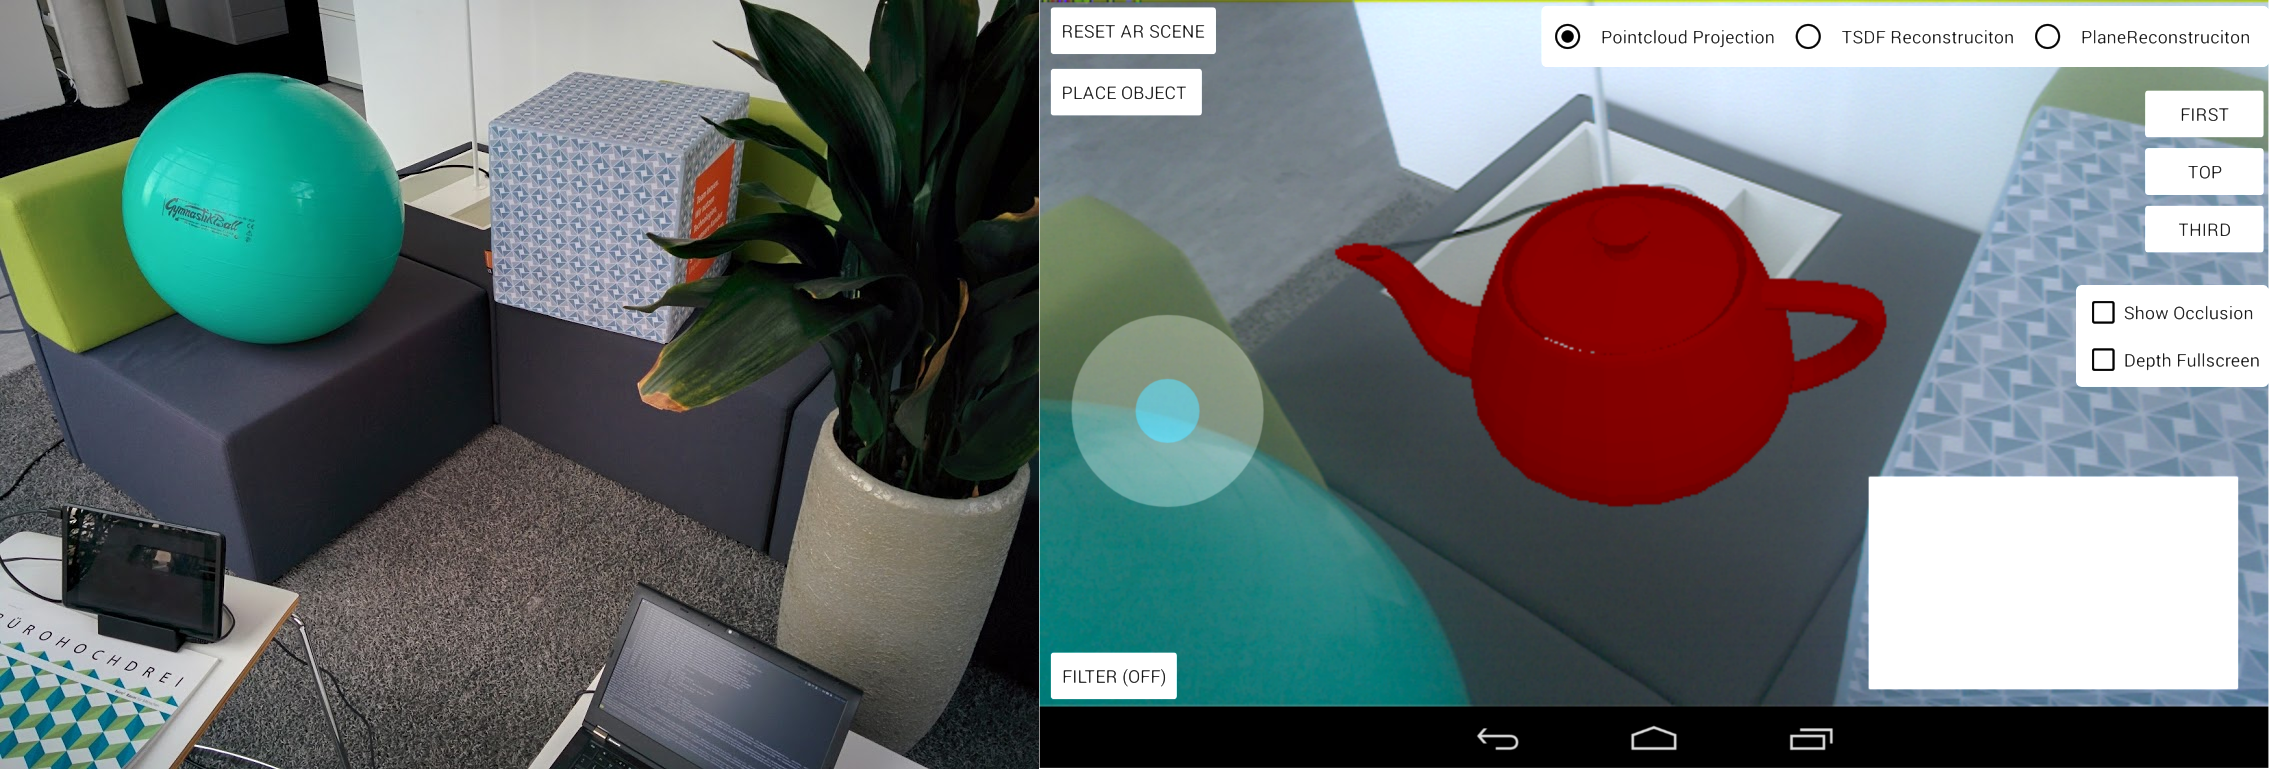
\includegraphics[width=1.0\textwidth]{content/images/evaluation/static-scene.png} 
  \caption{Links: Erste statische Szene mit einem Hocker und einem Sitzball. Rechts: Platzierung des virtuellen Objekts. }
  \label{fig:static-scene}
\end{figure}

Die zweite gewählte Szene, welche in Abbildung \ref{fig:plant-scene} links zu sehen ist, soll als Herausforderung die Überdeckung von komplexeren Strukturen testen. Sie besteht daher aus einer Pflanze, die sich, wie rechts im Bild zu sehen, vor dem virtuellen Objekt befindet. Auch hier befindet sich das Project Tango Gerät in einem Stativ, damit sich die Position während der Tests nicht ändert. 

\begin{figure}[h]
  \centering
	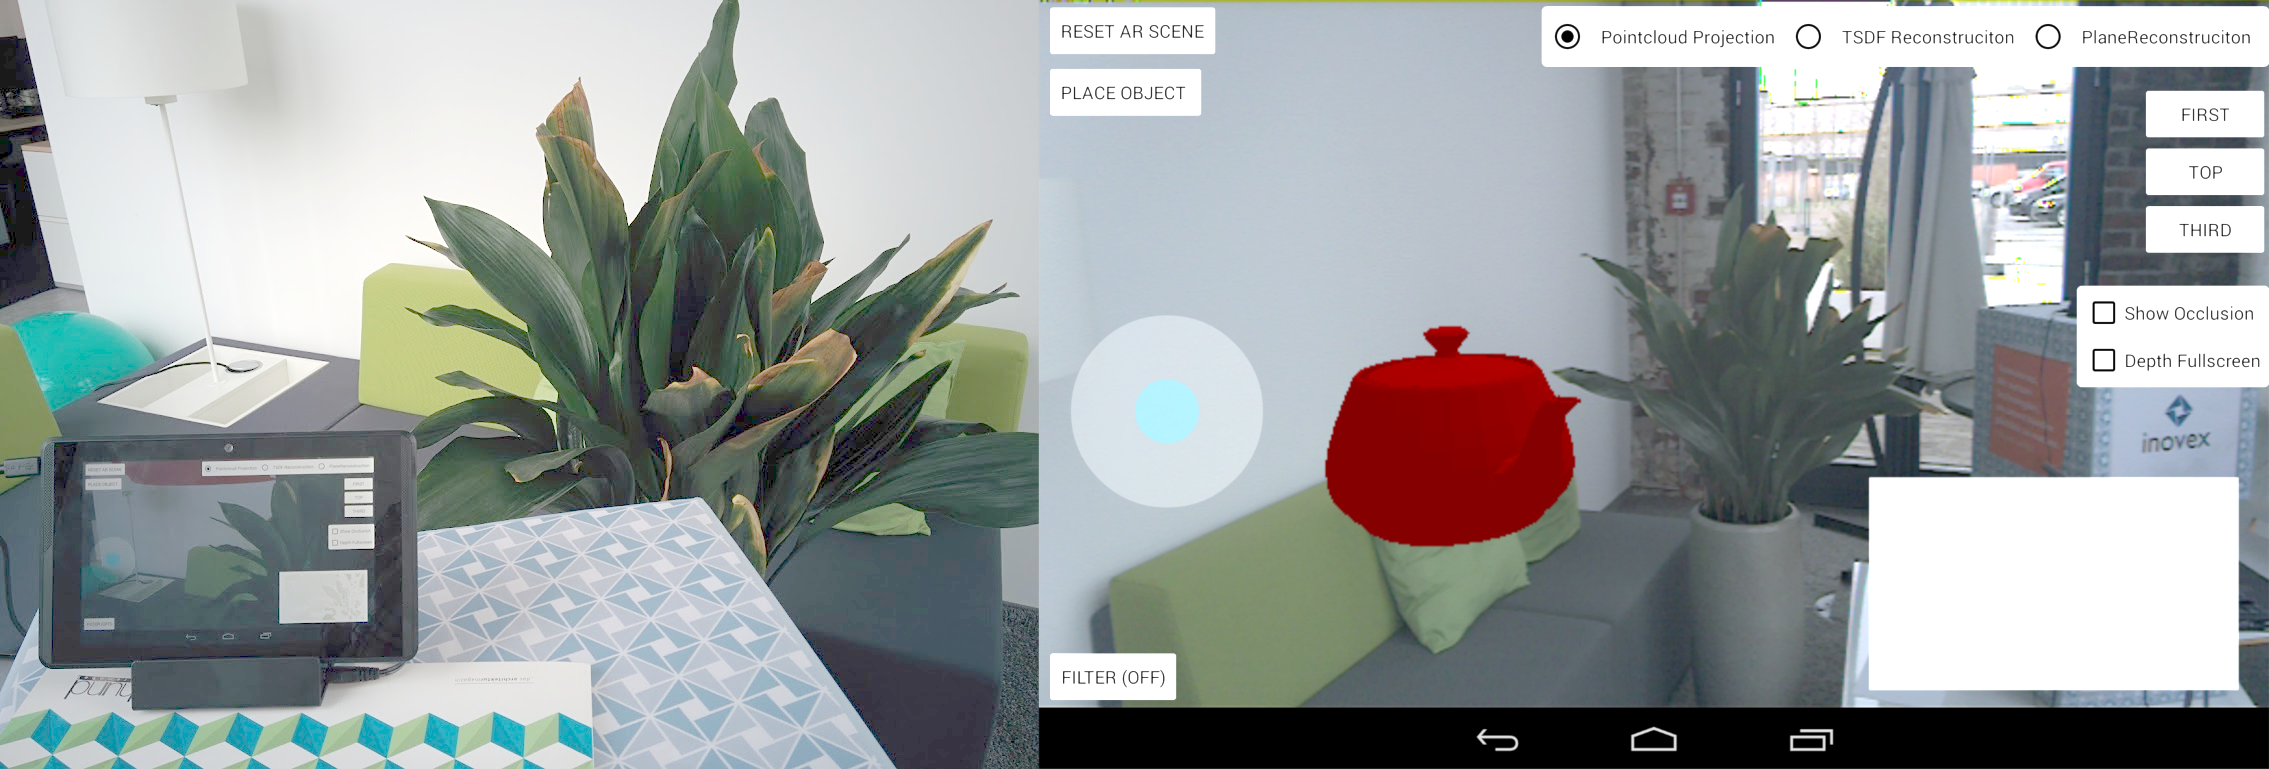
\includegraphics[width=1.0\textwidth]{content/images/evaluation/plant-scene.png} 
  \caption{Links: Zweite statische Szene mit einer Pflanze im Vordergrund. Rechts: Platzierung des virtuellen Objekts hinter der Pflanze. }
  \label{fig:plant-scene}
\end{figure}

Für beide Szenen sollen alle Kombinationen der Verfahren getestet werden. Somit ergeben sich sechs verschiedene Kombinationen pro Szene, in denen die Pointcloud Projektion, die TSDF Rekonstruktion und die Ebenenrekonstruktion jeweils mit und ohne der Anwendung des Guided Filter auf das Tiefenbild getestet werden. Für alle Kombinationen soll ein gerendertes Bild und ein Tiefenbild mit dem virtuellen Objekt festgehalten werden. Zur Auswertung werden die jeweils gerenderten Ergebnisbilder \(p\) mit einem manuell zugeschnittenem Ergebnisbild  \(q\) für jeden Pixel \(i\) verglichen. Für die Gegenüberstellung wird die Anzahl der abweichenden Pixel wie in Gleichung \ref{eq:diff} bestimmt. Ein Pixel wird nur als Veränderung gewertet, wenn die absolute Differenz der Pixel einen Faktor \(threshold\) übersteigt. Dies verhindert, dass leichte Variationen in der Farbintensität der Umgebung mit in die Wertung eingeht.

\begin{equation} \label{eq:diff}
d = \sum_i 
	\begin{cases}
		1, & \text{if } | p_i - q_i | > \text{threshold} \\
		0, & \textbf{otherwise}
	\end{cases}
\end{equation}

\section{Durchführung der Tests}

Die beiden Testszenen konnten wie beschrieben aufgebaut und mit allen Verfahren durchgetestet werden. Hierzu wurde mit der \enquote{Android Debug Bridge} (adb)\footnote{Android Debug Bridge - \url{http://goo.gl/ffH51x} (01.03.16)} eine Videoaufnahme gestartet, in der im Prototypen für jede Szene alle Verfahren durchgeschaltet wurden. Die Verfahren mussten dabei entsprechend zeitnah durchlaufen werden, um einen potentiellen Drift von Project Tangos Motion Tracking so minimal wie möglich zu halten. Denn dieser negative Effekt würden die Ergebnisse stark beeinträchtigen. 

Bei der Anwendung des Guided Filters wurde immer der Radius \(r = 24\) und der Einflussfaktor \(\epsilon = 0.8\) gewählt. Diese Werte versprachen nach einigen manuellen Tests erfolgreiche Ergebnisse. Der Radius wurde so groß gewählt, damit die bei den Rekonstruktionen üblichen Fehler auch weitreichend in den Gewichtungskernel berücksichtigt werden konnten. Abbildung \ref{fig:static_occlusion} und \ref{fig:plant_occlusion} im Anhang zeigen jeweils die aus dem Video extrahierten Bildausschnitte. Die obere Reihe zeigt die drei tiefengenerierenden Verfahren ohne den Guided Filter und die untere Reihe jeweils mit dem Filter. In der untersten Reihe sind jeweils die Projektionen der generierten Primitiven in der Szene zu sehen, um sich eine Vorstellung der Rekonstruktion machen zu können.

Nach der Ausführung dieser statischen Tests wurde jedes Verfahren zusätzlich mit einem bewegten Einsatz des Gerätes getestet. Dazu wurde das virtuelle Objekt zunächst neben einen Würfel gestellt, um danach das Gerät räumlich um den Würfel zu führen, sodass das virtuelle Objekt in der Bewegung überdeckt wurde. Da diese Tests aus zuvor beschriebenen Gründen nicht eindeutig reproduzierbar sind werden auch keine Testdaten hiervon erhoben. Dennoch soll diese nicht rein objektive Beobachtung während dieser Test mit in die Evaluation der Verfahren fließen.

\section{Auswertung der Ergebnisse}

Der Vergleich der Ergebnisse, welcher mit dem bereits beschriebenen Bilddifferenz Ansatz aus der Gleichung \ref{eq:diff} durchgeführt werden soll, wurde mit Hilfe der OpenCV Bibliothek durchgeführt und ist in Listing \ref{lst:compare} im Anhang zu finden. Für jede Szene wurde ein Referenzbild manuell konstruiert, welches dem idealen Ergebnis entsprechen soll. Zur Konstruktion der Vergleichsbilder wurden Ausschnitte mit leichten Anpassungen aus einigen Ergebnisbildern gewählt und zusammengeschnitten. Diese Referenzbilder sind in Abbildung \ref{fig:reference} oben zu finden. Mit dem Referenzbild wurden alle zuvor passend zugeschnitten Grafiken einer Szene verglichen. Außerdem wurde eine Maske für jede Szene für den Bereich des Ergebnisbildes bestimmt, der überhaupt für die Bestimmung der Differenz in Betracht gezogen wird. Die Masken sind jeweils in Abbildung \ref{fig:reference} unten zu finden.

\begin{figure}[h]
  \centering
	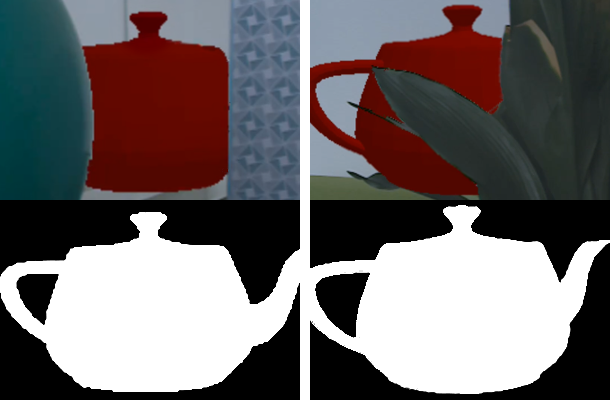
\includegraphics[width=0.7\textwidth]{content/images/evaluation/reference.png} 
  \caption{Manuell konstruierte Referenzbilder der idealen Überlagerung mit Filtermaske in Szene 1 (links) und 2 (rechts).}
  \label{fig:reference}
\end{figure}

Der gezeigte Skript zum Verglich der Ergebnisbilder mit den Referenzbildern ergibt neben den Differenzwerten, welche in Tabelle \ref{tab:results} zu finden sind, auch die absoluten Differenzbilder für jedes Verfahren. Diese Ergebnisbilder sind auch im Anhang in Abbildung \ref{fig:static_occlusion_results} zu finden. In der Abbildung werden beide Szenen mit je zwölf Bildern dargestellt, wobei jedes der drei Überlagerungsverfahren (horizontal) mit und ohne Anwendung des Guided Filter (vertikal) festgehalten sind. Sie sind also genau wie die Ergebnisse in Tabelle \ref{tab:results} angeordnet.


\begin{table}[h]
\centering
\begin{tabular}{@{}rrrr@{}}
\toprule
                      & \textbf{\begin{tabular}[c]{@{}r@{}}Pointcloud \\ Projektion\end{tabular}} & \textbf{\begin{tabular}[c]{@{}r@{}}TSDF \\ Rekonstruktion\end{tabular}} & \textbf{\begin{tabular}[c]{@{}r@{}}Ebenen \\ Rekonstruktion\end{tabular}} \\ \midrule
\textbf{Szene 1}      & 1400 & 3165 & 2193   \\
\textbf{Szene 1 + GF} & 1506 & 85 & 1545 \\
\textbf{Szene 2}      & 2478 & 4007 & 2180 \\
\textbf{Szene 2 + GF} & 67 & 1876 & 1529 \\
\bottomrule
\end{tabular}
\caption{Distanzwert zwischen dem Referenzbild und den Ergebnisbildern in der jeweiligen Szene}
\label{tab:results}
\end{table}
